\documentclass[sigconf,nonacm,screen,pbalance]{acmart}
\begin{document}
\title{Introduction to human-in-the-loop machine learning}
\author{Robert Monarch}
\maketitle

This chapter covers
\textbf{(1)} Annotating unlabeled data to create training, validation, and evaluation data.
\textbf{(2)} Sampling the most important unlabeled data items (active learning).
\textbf{(3)} Incorporating human–computer interaction principles into annotation.
\textbf{(4)} Implementing transfer learning to take advantage of information in existing models.

Unlike robots in the movies, most of today's artificial intelligence (AI) cannot learn by itself; instead, it relies on intensive human feedback. Probably 90\% of machine learning applications today are powered by supervised machine learning. This figure covers a wide range of use cases. An autonomous vehicle can drive you safely down the street because humans have spent thousands of hours telling it when its sensors are seeing a pedestrian, moving vehicle, lane marking, or other relevant object. Your in-home device knows what to do when you say ``Turn up the volume'' because humans have spent thousands of hours telling it how to interpret different commands. And your machine translation service can translate between languages because it has been trained on thousands (or maybe millions) of human-translated texts.

Compared with the past, our intelligent devices are learning less from programmers who are hardcoding rules and more from examples and feedback given by humans who do not need to code. These human-encoded examples--the training data--are used to train machine learning models and make them more accurate for their given tasks. But programmers still need to create the software that allows the feedback from nontechnical humans, which raises one of the most important questions in technology today: {\em What are the right ways for humans and machine learning algorithms to interact to solve problems}. After reading this book, you will be able to answer this question for many uses that you might face in machine learning.

Annotation and active learning are the cornerstones of human-in-the-loop machine learning. They specify how you elicit training data from people and determine the right data to put in front of people when you don't have the budget or time for human feedback on all your data. Transfer learning allows us to avoid a cold start, adapting existing machine learning models to our new task rather than starting at square one. We will introduce each of these concepts in this chapter.

\section{The basic principles of human-in-the-loop ML}
\emph{Human-in-the-loop machine learning}
is a set of strategies for combining human and machine intelligence in applications that use AI. The goal typically is to do one or more of the following:
\begin{itemize}
     \setlength{\itemindent}{-2em}
    \item Increase the accuracy of a machine learning model.
    \item Reach the target accuracy for a machine learning model faster.
    \item Combine human and machine intelligence to maximize accuracy.
    \item Assist human tasks with machine learning to increase efficiency. 
\end{itemize}

This book covers the most common active learning and annotation strategies and how to design the best interface for your data, task, and annotation workforce. The book gradually builds from simpler to more complicated examples and is written to be read in sequence. You are unlikely to apply all these techniques at the same time, however, so the book is also designed to be a reference for each specific technique.

\autoref{fig:f1} shows the human-in-the-loop machine learning process for adding labels to data. This process could be any labeling process: adding the topic to news stories, classifying sports photos according to the sport being played, identifying the sentiment of a social media comment, rating a video on how explicit the content is, and so on. In all cases, you could use machine learning to automate some of the process of labeling or to speed up the human process. In all cases, using best practices means implementing the cycle shown in \autoref{fig:f1}: sampling the right data to label, using that data to train a model, and using that model to sample more data to annotate.

\begin{figure}[ht]
\centering
\vspace{-5pt}
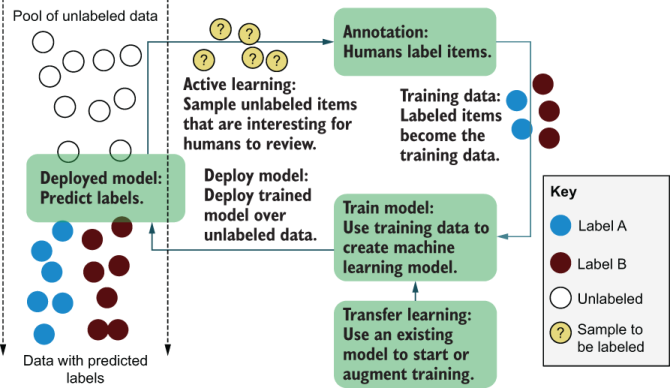
\includegraphics[width=\columnwidth]{CH01_F01_Munro.png}
\vspace{-20pt}
\caption{A mental model of the human-in-the-loop process for predicting labels on data}
\vspace{-10pt}
\label{fig:f1}
\end{figure}

In some cases, you may want only some of the techniques. If you have a system that backs off to a human when the machine learning model is uncertain, for example, you would look at the relevant chapters and sections on uncertainty sampling, annotation quality, and interface design. Those topics still represent the majority of this book even if you aren't completing the ``loop.''

This book assumes that you have some familiarity with machine learning. Some concepts are especially important for human-in-the-loop systems, including deep understanding of softmax and its limitations. You also need to know how to calculate accuracy with metrics that take model confidence into consideration, calculate chance-adjusted accuracy, and measure the performance of machine learning from a human perspective. (The appendix contains a summary of this knowledge.)

\section{Introducing annotation}

\emph{Annotation} is the process of labeling raw data so that it becomes training data for machine learning. Most data scientists will tell you that they spend much more time curating and annotating datasets than they spend building the machine learning models. Quality control for human annotation relies on more complicated statistics than most machine learning models do, so it is important to take the necessary time to learn how to create quality training data.

\subsection{Simple and more complicated annotation strategies}

An annotation process can be simple. If you want to label social media posts about a product as positive, negative, or neutral to analyze broad trends in sentiment about that product, for example, you could build and deploy an HTML form in a few hours. A simple HTML form could allow someone to rate each social media post according to the sentiment option, and each rating would become the label on the social media post for your training data.

An annotation process can also be complicated. If you want to label every object in a video with a bounding box, for example, a simple HTML form is not enough; you need a graphical interface that allows annotators to draw those boxes, and a good user experience might take months of engineering hours to build.

\subsection{Plugging the gap in data science knowledge}
Your machine learning algorithm strategy and your data annotation strategy can be optimized at the same time. The two strategies are closely intertwined, and you often get better accuracy from your models faster if you have a combined approach. Algorithms and annotation are equally important components of good machine learning.

All computer science departments offer machine learning courses, but few offer courses on creating training data. At most, you might find one or two lectures about creating training data among hundreds of machine learning lectures across half a dozen courses. This situation is changing, but slowly. For historical reasons, academic machine learning researchers have tended to keep the datasets constant and evaluated their research only in terms of different algorithms.

By contrast with academic machine learning, it is more common in industry to improve model performance by annotating more training data. Especially when the nature of the data is changing over time (which is also common), using a handful of new annotations can be far more effective than trying to adapt an existing model to a new domain of data. But far more academic papers focus on how to adapt algorithms to new domains {\em without} new training data than on how to annotate the right new training data efficiently.

Because of this imbalance in academia, I've often seen people in industry make the same mistake. They hire a dozen smart PhDs who know how to build state-of-the-art algorithms but don't have experience creating training data or thinking about the right interfaces for annotation. I saw exactly this situation recently at one of the world's largest auto manufacturers. The company had hired a large number of recent machine learning graduates, but it couldn't operationalize its autonomous vehicle technology because the new employees couldn't scale their data annotation strategy. The company ended up letting that entire team go. During the aftermath, I advised the company how to rebuild its strategy by using algorithms and annotation as equally-important, intertwined components of good machine learning.

\subsection{Quality human annotation: Why is it hard?}
To those who study it, annotation is a science that's tied closely to machine learning. The most obvious example is that the humans who provide the labels can make errors, and overcoming these errors requires surprisingly sophisticated statistics.

Human errors in training data can be more or less important, depending on the use case. If a machine learning model is being used only to identify broad trends in consumer sentiment, it probably won't matter whether errors propagate from 1\% bad training data. But if an algorithm that powers an autonomous vehicle doesn't see 1\% of pedestrians due to errors propagated from bad training data, the result will be disastrous. Some algorithms can handle a little noise in the training data, and random noise even helps some algorithms become more accurate by avoiding overfitting. But human errors tend not to be random noise; therefore, they tend to introduce irrecoverable bias into training data. No algorithm can survive truly bad training data.

For simple tasks, such as binary labels on objective tasks, the statistics are fairly straightforward for deciding which label is correct when different annotators disagree. But for subjective tasks, or even objective tasks with continuous data, no simple heuristics exist for deciding the correct label. Think about the critical task of creating training data by putting a bounding box around every pedestrian recognized by a self-driving car. What if two annotators have slightly different boxes? Which box is the correct one? The answer is not necessarily either box or the average of the two boxes. In fact, the best way to aggregate the two boxes is to use machine learning.

One of the best ways to ensure quality annotations is to ensure you have the right people making those annotations. Chapter 7 of this book is devoted to finding, teaching, and managing the best annotators. For an example of the importance of the right workforce combined with the right technology, see the following sidebar.

\textbf{Human insights and scalable machine learning equal production AI}
\emph{Expert anecdote by Radha Ramaswami Basu}
The outcome of AI is heavily dependent on the quality of the training data that goes into it. A small UI improvement like a magic wand to select regions in an image can realize large efficiencies when applied across millions of data points in conjunction with well-defined processes for quality control. An advanced workforce is the key factor: training and specialization increase quality, and insights from an expert workforce can inform model design in conjunction with domain experts. The best models are created by a constructive, ongoing partnership between machine and human intelligence.

We recently took on a project that required pixel-level annotation of the various anatomic structures within a robotic coronary artery bypass graft (CABG) video. Our annotation teams are not experts in anatomy or physiology, so we implemented teaching sessions in clinical knowledge to augment the existing core skills in 3D spatial reasoning and precision annotation, led by a solutions architect who is a trained surgeon. The outcome for our customer was successful training and evaluation data. The outcome for us was to see people from under-resourced backgrounds in animated discussion about some of the most advanced uses of AI as they quickly became experts in one of the most important steps in medical image analysis.

\emph{Radha Basu is founder and CEO of iMerit. iMerit uses technology and an AI workforce consisting of 50\% women and youth from underserved communities to create advanced technology workers for global clients. Radha previously worked at HP, took Supportsoft public as CEO, and founded the Frugal Innovation Lab at Santa Clara University.}

\section{Introducing active learning: Improving the speed and reducing the cost of training data}
Supervised learning models almost always get more accurate with more labeled data. \emph{Active learning} is the process of deciding which data to sample for human annotation. No one algorithm, architecture, or set of parameters makes one machine learning model more accurate in all cases, and no one strategy for active learning is optimal across all use cases and datasets. You should try certain approaches first, however, because they are more likely to be successful for your data and task.

Most research papers on active learning focus on the number of training items, but speed can be an even more important factor in many cases. In disaster response, for example, I have often deployed machine learning models to filter and extract information from emerging disasters. Any delay in disaster response is potentially critical, so getting a usable model out quickly is more important than the number of labels that need to go into that model.

\subsection{Three broad active learning sampling strategies: Uncertainty, diversity, and random}
Many active learning strategies exist, but three basic approaches work well in most contexts: uncertainty, diversity, and random sampling. A combination of the three should almost always be the starting point.

Random sampling sounds the simplest but can be the trickiest. What is random if your data is prefiltered, when your data is changing over time, or if you know for some other reason that a random sample will not be representative of the problem you are addressing? These questions are addressed in more detail in the following sections. Regardless of the strategy, you should always annotate some amount of random data to gauge the accuracy of your model and compare your active learning strategies with a baseline of randomly selected items.

Uncertainty and diversity sampling go by various names in the literature. They are often referred to as \emph{exploitation} and \emph{exploration}, which are clever names that alliterate and rhyme, but are not otherwise very transparent.

\paragraph{\bf\em Uncertainty sampling}
is the set of strategies for identifying unlabeled items that are near a decision boundary in your current machine learning model. If you have a binary classification task, these items will have close to a 50\% probability of belonging to either label; therefore, the model is called uncertain or confused. These items are most likely to be wrongly classified, so they are the most likely to result in a label that differs from the predicted label, moving the decision boundary after they have been added to the training data and the model has been retrained.

\paragraph{\bf\em Diversity sampling}
is the set of strategies for identifying unlabeled items that are
underrepresented or unknown to the machine learning model in its current state. The
items may have features that are rare in the training data, or they might represent
real-world demographics that are currently under-represented in the model. In either
case, the result can be poor or uneven performance when the model is applied, especially
when the data is changing over time. The goal of diversity sampling is to target new,
unusual, or underrepresented items for annotation to give the machine learning algorithm
a more complete picture of the problem space.

Although
the term \emph{uncertainty sampling} is widely used, \emph{diversity sampling} goes by
different names in different fields, such as representative sampling, stratified
sampling, outlier detection, and anomaly detection. For some use cases, such as
identifying new phenomena in astronomical databases or detecting strange network
activity for security, the goal of the task is to identify the outlier or anomaly, but
we can adapt them here as a sampling strategy for active learning.

Uncertainty
sampling and diversity sampling have shortcomings in isolation (\autoref{fig:f2}). Uncertainty
sampling might focus on one part of the decision boundary, for example, and diversity
sampling might focus on outliers that are a long distance from the boundary. So the
strategies are often used together to find a selection of unlabeled items that will
maximize both uncertainty and diversity.

\begin{figure}[ht]
\centering
% \vspace{-10pt}
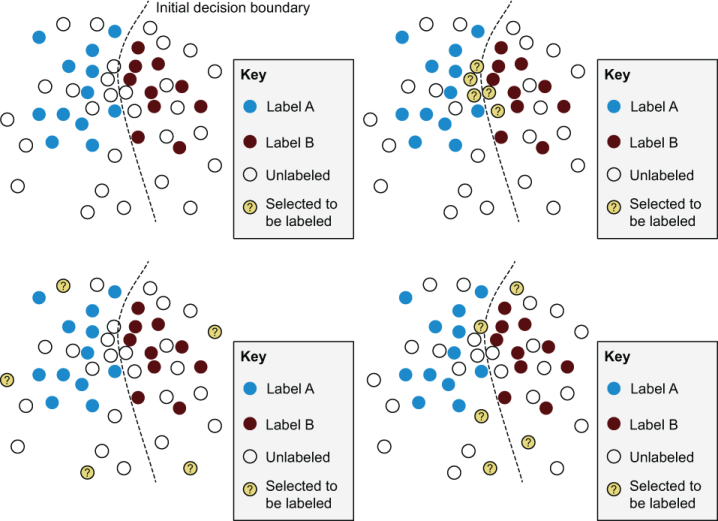
\includegraphics[width=\columnwidth]{CH01_F02_Munro.png}
\vspace{-20pt}
\caption{Pros and cons of different active learning strategies. Top left: The decision
boundary from a machine learning algorithm between items, with some items labeled A and
some labeled B. Top right: One possible result from uncertainty sampling. This active
learning strategy is effective for selecting unlabeled items near the decision boundary.
These items are the most likely to be wrongly predicted, and therefore, the most likely
to get a label that moves the decision boundary. If all the uncertainty is in one part
of the problem space, however, giving these items labels will not have a broad effect on
the model. Bottom left: One possible result of diversity sampling. This active learning
strategy is effective for selecting unlabeled items in different parts of the problem
space. If the diversity is away from the decision boundary, however, these items are
unlikely to be wrongly predicted, so they will not have a large effect on the model when
a human gives them a label that is the same as the model predicted. Bottom right: One
possible result from combining uncertainty sampling and diversity sampling. When the
strategies are combined, items are selected that are near diverse sections of the
decision boundary. Therefore, we are optimizing the chance of finding items that are
likely to result in a changed decision boundary.}
\vspace{-15pt}
\label{fig:f2}
\end{figure}

It
is important to note that the active learning process is iterative. In each iteration of
active learning, a selection of items is identified and receives a new human-generated
label. Then the model is retrained with the new items, and the process is repeated.
\autoref{fig:f3} shows two iterations for selecting and annotating new items, resulting in a
changing boundary.

\begin{figure}[ht]
\centering
% \vspace{-10pt}
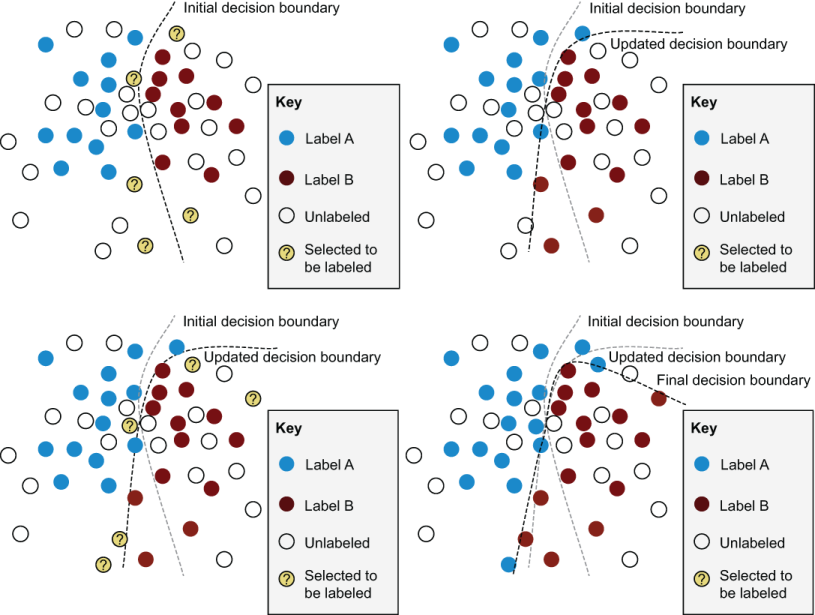
\includegraphics[width=\columnwidth]{CH01_F03_Munro.png}
\vspace{-20pt}
\caption{The iterative active learning process. \emph{Top left to bottom right}: Two
iterations of active learning. In each iteration, items are selected along a diverse
selection of the boundary, which in turn causes the boundary to move after retraining,
resulting in a more accurate machine learning model. Ideally, we requested human labels
for the minimum number of items as part of our active learning strategy. This request
speeds the time to get an accurate model and reduces the overall cost of human
annotation.}
\vspace{-20pt}
\label{fig:f3}
\end{figure}

Iteration
cycles can be a form of diversity sampling in themselves. Imagine that you used only
uncertainty sampling, and sampled from only one part of the problem space in an
iteration. You might solve all uncertainty in that part of the problem space; therefore,
the next iteration would concentrate somewhere else. With enough iterations, you might
not need diversity sampling at all. Each iteration from uncertainty sampling would focus
on a different part of the problem space, and together, the iterations are enough to get
a diverse sample of items for training.

Implemented
properly, active learning has this self-correcting function: each iteration finds new
aspects of the data that are best for human annotation. If some part of your data space
is inherently ambiguous, however, each iteration could keep bringing you back to the
same part of the problem space with those ambiguous items. So it is generally wise to
consider both uncertainty and diversity sampling strategies to ensure that you are not
focusing all your labeling efforts on a part of the problem space that your model might
not be able to solve.

\autoref{fig:f2} and \ref{fig:f3} give you good intuition about the process for active learning. As anyone who
has worked with high-dimensional or sequence data knows, it is not always
straightforward to identify distance from a boundary or diversity. At least, the process
is more complicated than the simple Euclidean distance in \autoref{fig:f2} and \ref{fig:f3}. But the
same idea still applies: we are trying to reach an accurate model as quickly as possible
with as few human labels as possible.

The
number of iterations and the number of items that need to be labeled within each
iteration depend on the task. When you're working in adaptive machine+human translation,
a single translated sentence is enough training data to require the model to update,
ideally within a few seconds. It is easy to see why from a user-experience perspective.
If a human translator corrects the machine prediction for some word, but the machine
doesn't adapt quickly, the human may need to (re)correct that machine output hundreds of
times. This problem is common when you're translating words that are highly
context-specific. You may want to translate a person's name literally in a news article,
for example, but translate it into a localized name in a work of fiction. The user
experience will be bad if the software keeps making the same mistake so soon after a
human has corrected it, because we expect recency to help with adaptation.

On
the technical side, of course, it is much more difficult to adapt a model quickly.
Consider large machine translation models. Currently, it takes a week or more to train
these models. From the experience of the translator, a software system that can adapt
quickly is employing continuous learning. In most use cases I've worked on, such as
identifying the sentiment in social media comments, I needed to iterate only every month
or so to adapt to new data. Although few applications have real-time adaptive machine
learning today, more are moving this way.

\subsection{What is a random selection of evaluation data?}
It
is
easy to \emph{say} that you should always evaluate on a random sample of held-out data,
but in practical terms, it is rarely easy to ensure that you have a truly random sample
of data. If you prefiltered the data that you are working with by keyword, time, or some
other factor, you already have a nonrepresentative sample. The accuracy of that sample
is not necessarily indicative of the accuracy on the data where your model will be
deployed.

I've
seen people use the well-known ImageNet dataset and apply machine learning models to a
broad selection of data. The canonical ImageNet dataset has 1,000 labels, each of which
describes the category of that image, such as ``Basketball,'' ``Taxi,'' or ``Swimming.'' The
ImageNet challenges evaluated held-out data from that dataset, and systems achieved
near-human-level accuracy within that dataset. If you apply those same models to a
random selection of images posted on a social media platform, however, accuracy
immediately drops to something like 10\%.

In
most applications of machine learning, the data will change over time as well. If you're
working with language data, the topics that people talk about will change over time, and
the languages themselves will innovate and evolve. If you're working with computer
vision data, the types of objects that you encounter will change over time. Equally
important, the images themselves will change based on advances and changes in camera
technology.

If
you can't define a meaningful random set of evaluation data, you should try to define a
\emph{representative} evaluation dataset.
If you define a representative dataset, you are admitting that a truly random sample
isn't possible or meaningful for your dataset. It is up to you to define what is
representative for your use case, based on how you are applying the data. You may want
to select data points for every label that you care about, a certain number from every
time period or a certain number from the output of a clustering algorithm to ensure
diversity. (I discuss this topic more in ch 4.)

You
may also want to have multiple evaluation datasets that are compiled through different
criteria. One common strategy is to have one dataset drawn from the same data as the
training data and at least one out-of-domain evaluation dataset drawn from a different
source. Out-of-domain datasets are often drawn from different types of media or
different time periods. If all the training data for a natural language processing (NLP)
task comes from historical news articles, for example, an out-of-domain dataset might come
from recent social media data. For most real-world applications, you should use an
out-of-domain evaluation dataset, which is the best indicator of how well your model is
truly generalizing to the problem and not simply overfitting quirks of that particular
dataset. This practice can be tricky with active learning, however, because as soon as
you start labeling that data, it is no longer out-of-domain. If doing so is practical, I
recommend that you keep an out-of-domain dataset to which you {\em don't} apply active
learning. Then you can see how well your active learning strategy is generalizing the
problem, not simply adapting and overfitting to the domains that it encounters.

\subsection{When to use active learning}
You should
use active learning when you can annotate only a small fraction of your data and when
random sampling will not cover the diversity of data. This recommendation covers most
real-world scenarios, as the scale of the data becomes an important factor in many use
cases.

A
good example is the amount of data present in videos. Putting a bounding box around
every object in every frame of a video, for example, would be time-consuming. Suppose
that this video is of a self-driving car on a street with about 20 objects you care
about (cars, pedestrians, signs, and so on). At 30 frames a second, that's 30 frames *
60 seconds * 20 objects, so you would need to create {\em 36,000} boxes for one minute
of data! Even the fastest human annotator would need at least 12 hours to annotate one
minute's worth of data.

If
we run the numbers, we see how intractable this problem is. In the United States, people
drive an average of 1 hour per day, which means that people in the United States drive
95,104,400,000 hours per year. Soon, every car will have a video camera on the front to
assist with driving. So 1 year's worth of driving in the United States alone would take
60,000,000,000 hours to annotate. There are not enough people on Earth to
annotate the videos of drivers in the United States today, even if the rest of the world
did nothing but annotate data all day to make U.S. drivers safer.

So
any data scientists at an autonomous-vehicle company needs to answer a variety of
questions about the annotation process. Is every {\em n}th frame in a video OK? Can we
sample the videos so that we don't have to annotate them all? Are there ways to design
an interface for annotation to speed the process?

The
intractability of annotation is true in most situations. There will be more data to
annotate than there is budget or time to put each data point in front of a human. That's
probably why the task is using machine learning in the first place. If you have the
budget and time to annotate all the data points manually, you probably don't need to
automate the task.

You
don't need active learning in every situation, although human-in-the-loop learning
strategies might still be relevant. In some cases, humans are required by law to
annotate every data point, such as a court-ordered audit that requires a human to look
at every communication within a company for potential fraud. Although humans will
ultimately need to look at every data point, active learning can help them find the
fraud examples faster and determine the best user interface to use. It can also identify
potential errors with human annotations. In fact, this process is how many audits are
conducted today.

There
are also some narrow use cases in which you almost certainly don't need active learning.
If you are monitoring equipment in a factory with consistent lighting, for example, it
should be easy to implement a computer vision model to determine whether a given piece
of machinery is on or off from a light or switch on that machine. As the machinery,
lighting, camera, and the like are not changing over time, you probably don't need to
use active learning to keep getting training data after your model has been built. These
use cases are rare, however. Fewer than 1\% of the use cases that I have encountered in
industry have no use for more training data.

Similarly,
there might be use cases in which your baseline model is accurate enough for your
business use case or the cost of more training data exceeds any value that a more
accurate model might provide. This criterion could also be the stopping point for active
learning
iterations.

\section{ML and HCI}
For
decades,
a lot of smart people failed to make human translation faster and more accurate with the
help of machine translation. It seems obvious that it should be possible to combine
human translation and machine translation. As soon as a human translator needs to
correct one or two errors in a sentence from machine translation output, however, it
would be quicker for the translator to retype the whole sentence from scratch. Using the
machine translation sentence as a reference when translating makes little difference in
speed, and unless the human translator takes extra care, they will end up perpetuating
errors in the machine translation, making their translation less accurate.

The
eventual solution to this problem was not in the accuracy of the machine translation
algorithms, but in the user interface. Instead of requiring human translators to retype
whole sentences, modern translation systems let them use the same kind of predictive
text that has become common in phones and (increasingly) in email and document
composition tools. Human translators type translations as they always have, pressing
Enter or Tab to accept the next word in the predicted translation, increasing their
overall speed every time the machine translation prediction is correct. So the biggest
breakthrough was in human–computer interaction, not the underlying machine learning
algorithm.

Human–computer
interaction is an established field in computer science that has recently become
especially important for machine learning. When you are building interfaces for humans
to create training data, you are drawing on a field that is at the intersection of
cognitive science, social sciences, psychology, user-experience design, and several
other fields.

\subsection{UIs: How do you create training data?}
Often,
a
simple web form is enough to collect training data. The human–computer interaction
principles that underlie interaction with web forms are equally simple: people are
accustomed to web forms because they see them all day. The forms are intuitive because a
lot of smart people worked on and refined HTML forms. You are building on these
conventions: people know how a simple HTML form works, so you don't need to educate
them. On the other hand, breaking these conventions would confuse people, so you are
constrained to expected behavior. You might have some idea that dynamic text could speed
some task, but that convention could confuse more people than it helps.

The
simplest interface--binary responses--is also the best for quality control. If you can
simplify or break your annotation project into binary tasks, it is a lot easier to
design an intuitive interface and to implement the annotation quality control features
covered in chapters 8–11.

When
you are dealing with more complicated interfaces, the conventions also become more
complicated. Imagine that you are asking people to put polygons around certain objects
in an image, which is a common use case for autonomous-vehicle companies. What
modalities would an annotator expect? Would they expect freehand, lines, paintbrushes,
smart selection by color/region, or other selection tools? If people are accustomed to
working on images in programs such as Adobe Photoshop, they might expect the same
functionality when annotating images. In the same way that you are building on and
constrained by people's expectations for web forms, you are also constrained by their
expectations for selecting and editing images. Unfortunately, those expectations might
require hundreds of hours of coding to build if you are offering full-featured
interfaces.

For
anyone who is undertaking a repetitive task such as creating training data, moving a
mouse is inefficient and should be avoided if possible. If the entire annotation process
can happen on a keyboard, including the annotation itself and any form submissions or
navigations, the rhythm of the annotators will be greatly improved. If you have to
include a mouse, you should be getting rich annotations to make up for the slower
inputs.

Some
annotation tasks have specialized input devices. People who transcribe speech to text
often use foot pedals to navigate backward and forward in time in the audio recording.
The process allows them to leave their hands on the keyboard. Navigating a recording
with their feet is much more efficient than navigating the recording with a mouse.

Exceptions
such as transcription aside, the keyboard is still king. Most annotation tasks haven't
been popular for as long as transcription and therefore haven't developed specialized
input devices. For most tasks, using a keyboard on a laptop or PC is faster than using
the screen of a tablet or phone. It's not easy to type on a flat surface while keeping
your eyes on inputs, so unless a task is a simple binary selection task or something
similar, phones and tablets are not suited to high-volume data
annotation.

\subsection{Priming: What can influence human perception?}

To
get
accurate training data, you have to take into account the focus of the human annotator,
their attention span, and contextual effects that might cause them to make errors or to
otherwise change their behavior. Consider a great example from linguistics research. In
a study called ``Stuffed toys and speech perception'' (\href{https://doi.org/10.1515/ling.2010.027}{https://doi.org/10.1515/ling.2010.027}),
people were asked to distinguish between Australian and New Zealand accents. Researchers
placed a stuffed toy kiwi bird or kangaroo (iconic animals for those countries) on a
shelf in the room where participants undertook the study. The people who ran the study
did not mention the stuffed toy to the participants; the toy was simply in the
background. Incredibly, people interpreted an accent as sounding more New Zealand-like
when a kiwi bird was present and more Australia-like when a kangaroo was present. Given
this fact, it is easy to imagine that if you are building a machine learning model to
detect accents (perhaps you are working on a smart home device that you want to work in
as many accents as possible), you need to take context into account when collecting
training data.

When
the context or sequence of events can influence human perception, this phenomenon is
known as {\em priming} The most important type in creating training data is
\emph{repetition priming},
which occurs when the sequence of tasks can influence someone's perception. If an
annotator is labeling social media posts for sentiment, for example, and they encounter
99 negative sentiment posts in a row, they are more likely to make an error by labeling
the hundredth post as negative when it is positive. The post may be inherently ambiguous
(such as sarcasm) or a simple error caused by an annotator's fading attention during
repetitive work. In chapter 11, I talk about the types of priming you need to control for.

\subsection{The pros and cons of creating labels by evaluating machine learning predictions}
One
way
to combine machine learning and ensure quality annotations is to use a simple
binary-input form to have people evaluate a model prediction and confirm or reject that
prediction. This technique can be a nice way to turn a more complicated task into a
binary annotation task. You could ask someone whether a bounding box around an object is
correct as a simple binary question that doesn't involve a complicated editing/selection
interface. Similarly, it is easier to ask an annotator whether some word is a location
in a piece of text than it is to provide an interface to efficiently annotate phrases
that are locations in free text.

When
you do so, however, you run the risk of focusing on localized model uncertainty and
missing important parts of the problem space. Although you can simplify the interface
and annotation accuracy evaluation by having humans evaluate the predictions of machine
learning models, you still need a diversity strategy for sampling, even if that strategy
is merely ensuring that a random selection of items is also available.

\subsection{Basic principles for designing annotation interfaces}
Based
on
what I've covered so far, here are some basic principles for designing annotation
interfaces. I'll go into more detail on these principles throughout the
book:

\begin{itemize}
     \setlength{\itemindent}{-2em}
    \item Cast your problems as binary choices wherever possible.
    \item Ensure that expected responses are diverse to avoid priming.
    \item Use existing interaction conventions.
    \item Allow keyboard-driven responses.
\end{itemize}

\section{ML-assisted humans vs. human-assisted ML}

Human-in-the-loop
machine
learning can have two distinct goals: making a machine learning application more
accurate with human input and improving a human task with the aid of machine learning.
The two goals are sometimes combined, and machine translation is a good example. Human
translation can be made faster by using machine translation to suggest words or phrases
that a human can choose to accept or reject, much as your smartphone predicts the next
word as you are typing. This task is a machine-learning-assisted human processing task.
I've also worked with customers who use machine translation when human translation would
be too expensive. Because the content is similar across the human- and
machine-translated data, the machine translation system gets more accurate over time
from the data that is human-translated. These systems are hitting both goals, making the
humans more efficient and making the machines more accurate.

Search
engines are another great example of human-in-the-loop machine learning. People often
forget that search engines are a form of AI despite being so ubiquitous for general
search and for specific use cases such as e-commerce and navigation (online maps). When
you search for a page online and click the fourth link that comes up instead of the
first link, for example, you are probably training that search engine (information
retrieval system) that the fourth link might be a better top response for your search
query. There is a common misconception that search engines are trained only on feedback
from end users. In fact, all the major search engines employ thousands of annotators to
evaluate and tune their search engines. Evaluating search relevance is the single
largest use case for human annotation in machine learning. Although there has been a
recent rise in popularity of computer vision use cases, such as autonomous vehicles, and
speech use cases, such as in-home devices and smartphones, search relevance is still the
largest use case for professional human annotation.

However
they appear at first glance, most human-in-the-loop machine learning tasks have some
element of both machine-learning-assisted humans and human-assisted machine learning, so
you need to design for both.

\section{Transfer learning to kick-start your models}
You
don't
need to start building your training data from scratch in most cases. Often, existing
datasets are close to what you need. If you are creating a sentiment analysis model for
movie reviews, for example, you might have a sentiment analysis dataset from product
reviews that you can start with and then adapt to your use cases. This process--taking a
model from one use case and adapting it to another--is known as transfer learning.

Recently,
there has been a large increase in the popularity of adapting general pretrained models
to new, specific use cases. In other words, people are building models
\emph{specifically} to be used in transfer learning for many use cases. These models are
often referred to as {\em pretrained} models.

Historically,
transfer learning has involved feeding the outputs of one process into another. An
example in NLP might be
\begin{quote}
{\em General part-of-speech tagger $\rightarrow$ Syntactic parser $\rightarrow$ Sentiment analysis tagger}
\end{quote}

Today, transfer learning typically means
\begin{quote}
{\em Retraining
part of a neural model to adapt to a new task (pretrained models) or using the
parameters of one neural model as inputs to another}
\end{quote}

\autoref{fig:f4} shows an example of transfer learning. A model can be trained on one set of labels
and then retrained on another set of labels by keeping the architecture the same and
freezing part of the model, retraining only the last layer in this case.

\begin{figure}[ht]
\centering
\vspace{-5pt}
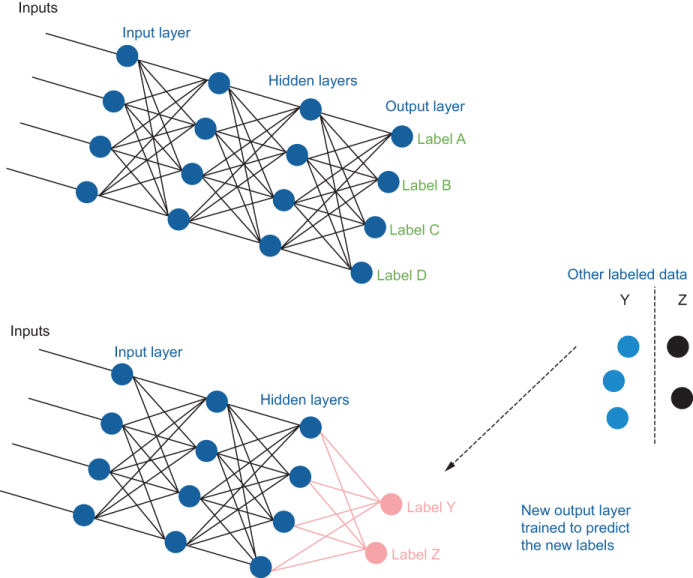
\includegraphics[width=\columnwidth]{CH01_F04_Munro.png}
\vspace{-20pt}
\caption{An example of transfer learning. A model was built to predict a label as ``A,'' ``B,''
``C,'' or ``D.'' Retraining the last layer of the model and using far fewer human-labeled
items than if we were training a model from scratch, the model is able to predict labels
``Y'' and ``Z.''}
\vspace{-15pt}
\label{fig:f4}
\end{figure}

\subsection{Transfer learning in computer vision}
Transfer
learning
has seen the most progress recently in computer vision. A popular strategy is to start
with the ImageNet dataset and build a model from the millions of examples to classify
the 1,000 labels: sports, birds, human-made objects, and so on.

To
learn to classify different types of sports, animals, and objects, the machine learning
model is learning about the types of textures and edges that are needed to distinguish
1,000 types of items in images. Many of these textures and edges are more general than
the 1,000 labels and can be used elsewhere. Because all the textures and edges are
learned in the intermediate layers of the network, you can retrain only the last layer
on a new set of labels. You may need only a few hundred or a few thousand examples for
each new label, instead of millions, because you are already drawing on millions of
images for the textures and edges. ImageNet has seen high success when people have
retrained the final layer to new labels with little data, including objects such as
cells in biology and geographic features from satellite views.

It
is also possible to retrain several layers instead of the last one and to add more
layers to the model from which you are transferring. Transfer learning can be used with
many architectures and parameters to adapt one model to a new use case, but with the
same goal of limiting the number of human labels needed to build an accurate model on
new data.

Computer
vision has been less successful to date for moving beyond image labeling. For tasks such
as detecting objects within an image, it is difficult to create transfer learning
systems that can adapt from one type of object to another. The problem is that objects
are being detected as collections of edges and textures rather than as whole objects.
Many people are working on the problem, however, so there is no doubt that breakthroughs
will occur.

\subsection{Transfer learning in NLP}
The
big
push for pretrained models for NLP is even more recent than for computer vision.
transfer learning of this form has become popular for NLP only in the past two or three
years, so it is one of the most cutting-edge technologies covered in this text, but it
also might become out of date quickly.

ImageNet-like
adaptation does not work for language data. Transfer learning for one sentiment analysis
dataset to another sentiment analysis dataset provides an accuracy increase of only
\textasciitilde 2–3\%. Models that predict document-level labels don't capture the breadth of human
language to the extent that equivalent computer vision models capture textures and
edges. But you can learn interesting properties of words by looking at the contexts in
which they occur regularly. Words such as {\em doctor} and {\em surgeon} might occur
in similar contexts, for example. Suppose that you found 10,000 contexts in which any
English word occurs, looking at the set of words before and after. You can see how
likely the word {\em doctor} is to occur in each of these 10,000 contexts. Some of
these contexts will be medical-related, so {\em doctor} will have a high score in those
contexts. But most of the 10,000 contexts will not be medical-related, so {\em doctor}
will have a low score in those contexts. You can treat these 10,000 scores like a
10,000-long vector. The word {\em surgeon} is likely to have a vector similar to that
of {\em doctor} because it often occurs in the same context.

The
concept of understanding a word by its context is old and forms the basis of functional
theories of linguistics:

{\em You shall know a word by the company it keeps (Firth, J. R. 1957:11)}

Strictly,
we need to go below the word to get to the most important information. English is an
outlier in that words tend to make good atomic units for machine learning. English
allows for complex words such as {\em un-do-ing} it is obvious why we would want to
interpret the separate parts (morphemes), but English does this much more rarely than a
typical language. What English expresses with word order, such as subject-verb-object,
is more frequently expressed with affixes that English limits to things such as present
and past tense and singular/plural distinctions. So for machine learning tasks that are
not biased toward a privileged language such as English, which is an outlier, we need to
model subwords.

Firth
would appreciate this fact. He founded England's first linguistics department at SOAS,
where I worked for two years helping record and preserve endangered languages. It was
clear from my time there that the full breadth of linguistic diversity means that we
need more fine-grained features than words alone. Human-in-the-loop machine learning
methods are necessary if we are going to adapt the world's machine-learning capabilities
to as many of the 7,000 world languages as possible.

When
transfer learning had its recent breakthrough moment, it followed the principle of
understanding words (or word segments) in context. We can get millions of labels for our
models for free if we predict the word from its context:

{\em My \_\_\_ is cute. He \_\_\_ play-ing}

No
human labeling is required. We can remove some percentage of the words in raw text and
then turn the remaining text into a predictive machine-learning task. As you can guess,
the first blank word might be {\em dog}, {\em puppy}, or {\em kitten}, and the second
blank word is likely to be {\em is} or {\em was} As with {\em surgeon} and
{\em doctor} we can predict words from context.

Unlike
the early example in which transfer learning from one type of sentiment to another
failed, these kinds of pretrained models have been widely successful. With only minor
tuning from a model that predicts a word in context, it is possible to build
state-of-the-art systems with small amounts of human labeling for language tasks such as
question answering, sentiment analysis, and textual entailment. Unlike computer vision,
transfer learning is quickly becoming ubiquitous for complicated NLP tasks such as
summarization and translation.

The
pretrained models are not complicated. The most sophisticated ones today are trained to
predict a word in context, the order of words in a sentence, and the order of sentences.
From that baseline model of three types of predictions that are inherent in the data, we
can build almost any NLP use case with a head start. Because word order and sentence
order are inherent properties of the documents, the pretrained models don't need human
labels. They are still built like supervised machine learning tasks, but the training
data is generated for free. The models might be asked to predict one in every ten words
that have been removed from the data and to predict when certain sentences follow each
other in the source documents, providing a powerful head start before any human labels
are required for your task.

Pretrained
models, however, are limited by how much unlabeled text is available. Much more
unlabeled text is available in English than in other languages, even when you take the
overall frequency of different languages into account. There will be cultural biases,
too. The example {\em My dog is cute} might appear frequently in online text, which is
the main source of data for pretrained models. But not everyone has a dog as a pet. When
I briefly lived in the Amazon to study the Matsés language, monkeys were popular pets.
The English phrase {\em My monkey is cute} rarely appears online, and the Matsés
equivalent {\em Chuna bëdambo ikek} doesn't occur at all. Word vectors and the
contextual models in pretrained systems do allow multiple meanings to be expressed by
one word, so they could capture both {\em dog} and {\em monkey}. in this context, but
they are still biased toward the data on which they are trained, and the {\em monkey}
context is unlikely to occur in large volumes in any language. We need to be aware that
pretrained systems will tend to amplify cultural biases.

Pretrained
models still require additional human labels to achieve accurate results in their tasks,
so transfer learning does not change our general architecture for human-in-the-loop
machine learning. It can give us a substantial head start in labeling, however, which
can influence the choice of active learning strategy that we use to sample additional
data items for human annotation and even the interface by which humans provide that
annotation.

Transfer
learning also forms the basis of some of the advanced active learning strategies
discussed in chapter 5 and the advanced data annotation and augmentation strategies in
chapter
9.

\section{What to expect in this text}
To
think
about how the pieces of this text fit together, it can be useful to think of the topics
in terms of a knowledge quadrant (\autoref{fig:f5}).

\begin{figure}[ht]
\centering
\vspace{-5pt}
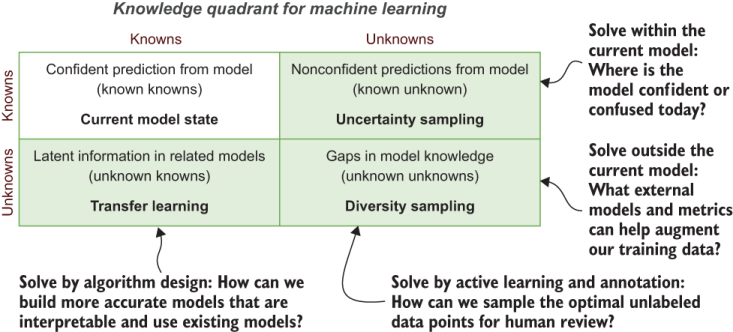
\includegraphics[width=\columnwidth]{CH01_F05_Munro.png}
\vspace{-20pt}
\caption{A machine learning knowledge quadrant, covering the topics in this book and
expressing them in terms of what is known and unknown for your machine learning models}
\vspace{-10pt}
\label{fig:f5}
\end{figure}

\noindent{\bf The four quadrants are}

\noindent{\bf K K:} What
your machine learning model can confidently and accurately do today. This quadrant
is your model in its current state.

\noindent{\bf K u:} What
your machine learning model cannot confidently do today. You can apply uncertainty
sampling to these items.

\noindent{\bf u K:} Knowledge
within pretrained models that can be adapted to your task. Transfer learning allows
you to use this knowledge.

\noindent{\bf u u:} Gaps
in your machine learning model. You can apply diversity sampling to these items.

The
columns and rows are meaningful too, with the rows capturing knowledge of your model in
its current state and the columns capturing the type of solutions needed:
\begin{itemize}
    \item 
    The top row captures your model's knowledge.
    \item 
    The bottom row captures knowledge outside your model.
    \item 
    The left column can be addressed by the right algorithms.
    \item 
    The right column can be addressed by human interaction.
\end{itemize}
This
text covers a wide range of technologies, so it might help to keep this figure handy to
know where everything fits in.

The
book has cheat sheets at the end of the first few chapters as a quick reference for the
major concepts that were covered. You can keep these cheat sheets handy while reading
later chapters.

\section{Summary}

The
broader human-in-the-loop machine learning architecture is an iterative process
combining human and machine components. Understanding these components explains how the
parts of this book come together.

You
can use some basic annotation techniques to start creating training data. Understanding
these techniques ensures that you are getting annotations accurately and efficiently.

The
two most common active learning strategies are uncertainty sampling and diversity
sampling. Understanding the basic principles of each type helps you strategize about the
right combination of approaches for your particular problems.

Human–computer
interaction gives you a framework for designing the user-experience components of
human-in-the-loop machine learning systems.

Transfer
learning allows us to adapt models trained from one task to another and build more
accurate models with fewer annotations.

\section{Check your understanding}

{\bf What is an example of transfer learning in NLP?}
Transfer
learning in NLP is exemplified by using
pretrained models for language tasks such as question answering,
sentiment analysis, and textual entailment.

{\bf What is the criterion for stopping active learning iterations?}
The
criterion for stopping active learning iterations is when the cost of
more training data exceeds any value that a more accurate model might
provide.

{\bf What is an example of a human-in-the-loop machine learning task?}
Search
engine relevance evaluation is an example of a human-in-the-loop machine
learning task.

{\bf What is the main breakthrough that allowed for the combination of human translation and machine translation?}
The
main breakthrough that allowed for the combination of human translation
and machine translation was HCI.

{\bf What are the principles that underlie interaction with web forms?}
The
principles that underlie interaction with web forms are to use existing
interaction conventions.

{\bf What is the main purpose of transfer learning for NLP?}
The
main purpose of transfer learning for NLP is to predict words in
context.

{\bf What is an example of a human-in-the-loop machine learning task?}
Search
engine relevance evaluation is an example of a human-in-the-loop machine
learning task.

{\bf What is transfer learning?}
Transfer learning is adapting a model trained from one task to another.

\end{document}
\endinput
